\section{Validierung}
Die Validierung der entwickelten Hardware-Abstraktionsschicht (HW\_API) dient dem Nachweis ihrer Funktionalität, Korrektheit und Plattformunabhängigkeit. 
Ziel dieser Untersuchung ist es zum einen sicherzustellen, dass die implementierten Klassen sowohl auf STM32- als auch auf ESP32-Plattformen zuverlässig arbeiten und den gestellten Anforderungen entsprechen, zum anderen zu vergleichen, welche Änderungen die neue Zwischenschicht bezüglich Ressourcenverbrauch mit sich bringt.

\subsection{Tests}
Die Überprüfung der Funktionalität wurden mehreren Schritten gewährleistet.
So musste zunächst bestätigt werden, dass der Code fehlerfrei kompiliert und gebaut wird.
Beim Debuggen musste festgestellt werden, ob das Programm sich so verhält, wie es erwartet ist oder ob unerwünschte Seiteneffekte auftreten.

\subsection*{Testaufbau}
Um die korrekte Funktionsweise der Gpio-Klasse zu gewährleisten wurde mit einem Breadboard eine Schaltung mit einem Taster und einer LED aufgebaut.
Diese konnte dann die verfügbaren \gls{mcu}s an den konfigurierten Pins angeschlossen werden.
Für die Steuerung der Schaltung wurde ein Programm implementiert, dass bei Betätigung des Tasters die LED zum leuchten bringt. 
Bei erneuter Betätigung sollte die LED wieder ausgeschalten werden.
Auf diese Weise sollte, wie zu Beginn gefordert, das Lese- und Schreibverhalten der neuen Klasse überprüft und bestätigt werden.

Um die Funktionsweise der SPI- und DMA-Klassen zu überprüfen, wurde jeweils ein Code für einen Master und ein Code für einen Slave implementiert.
Die Pinkonfiguration war für beide die identisch, indem für die Systemclock SCK, Master-Out-Slave-In MOSI, Master-In-Slave-Out MISO und NSS/CS Negative-Slave-Select bzw. Chip-Select jeweils ein Gpio-Objekt erstellt wurde.
Für jede Hardware wurde jeweils ein SPI-Objekt und ein DMA-Objekt erstellt.

Im Code wurde implementiert, dass der Master ein 'A' sendet und auf eine Antwort wartet, während der Slave ein 'O' sendet und eine Nachricht wartet.
Der Master-Code wurde auf ein STM32Nucleo-C031C6, der Slave-Code auf ein STM32Nucleo-G0B1RE geflasht. 
Die beiden MCUs wurden über die in der projct\_config.hpp definierte Gpio-Objekte mit einander verbunden.
An die einzelnen Pins wurden dann Klammern eines Oszilloskops angeschlossen um die Signale der einzelnen Pins (SCK, MOSI, MISO, NSS/CS) zu beobachten und mit sauberen Signalen eine Beispielprojekts aus der STM32CubeIDE zu vergleichen.
Damit sollte bestätigt werden, dass Kommunikation über den SPI-Bus mit den neuen Klassen funktionsfähig implementiert werden konnte. 

\subsection*{Testergebnisse}
\subsubsection{Struktur - Build, Flash, Erase, Debug}
% CMakeLists, Build, Compile
Beginnend mit der Auswahl der Hardware durch die Kombination von Makefilekonfigurationen (stm32\_config.mk bzw. esp\_config.mk), CMakeLists-Struktur und Factory-Imlpementierung konnte Schritt für Schritt eine Struktur erarbeitet werden, die im weiteren Verlauf erfolgreich funktioniert hat und verwendet wurde.
Zusätzlich bei unerwartetem Verhalten auch entsprechende Fehlermeldungen ausgab.
Im Fall der Auswahl der Hardware, hat neben dem Wechsel zwischen unterschiedlichen Familien, STM32C0xx und STM32G0xx, über die stm32\_config.mk auch der Wechsel zur verfügbaren ESP32C6-DevKit1 mit der esp32\_config.mk und dem Makefile erfolgreich funktioniert.
Der Einsatz von definierten Makros, wie beispielsweise \texttt{TARGET\_PLATFORM} \texttt{MCU\_FAMILY} oder \texttt{MCU\_SPECIFIC}, um in den CMakeLists.txt-Dateien die entsprechenden Bibliotheken auszuwählen, Dateien hinzuzufügen sowie Abschnitte freizuschalten, hat sich als vorteilhaft für die Erstellung eines automatisierten Kompilations- und Buildprozesses innerhalb der gesamten Struktur erwiesen.
Darüber hinaus hatte dies eine erfolgreiche Erstellung der Hardwareobjekte durch die Factory zur Folge.
Diese wählt anhand der Makros erst die richtige Plattform und im weiteren Verlauf die spezifische Hardware aus.
Sollte es im Compilier- oder Buildprozess zu Fehlern kommen, haben die Fehlermeldungen dabei geholfen die kritische Stelle zu identifizieren und das Problem beheben.
Sollte es dennoch zu tiefergreifenden Problemen kommen, konnte mit dem Befehlen \texttt{make stm32-reset}, \texttt{make esp32-reset}, \texttt{make stm32-erase} bzw. \texttt{make esp32-erase} der fehlerhafte Code entweder neugestartet oder gänzlich von der Hardware entfernt werden.
Mit den Befehl \texttt{make stm32-debug} konnte der Code Zeile für Zeile durchlaufen und Verhalten der Hardwareregister beobachtet werden um nachzuvollziehen ob die Werteänderungen dem erwarteten Verhalten entsprachen oder nicht.
% TODO: ESP32 Debug Problem
Lediglich der Befehl \texttt{make esp32-debug} sorgte für schwerwiegende Problem. 
Auch wenn die genannten restlichen Befehle, sowohl auf Seiten von STM32 als auch ESP32, funktioniert haben und sie im Laufe der Entwicklung regelmäßig Verwendung fanden, konnte nicht herausgefunden werden, woran es scheiterte ein Debug-Session für den ESP32-Code zu erstellen.

% GPIO
\subsubsection{GPIO}
Mit dem erstellten Programm, das die neuen Gpio-Objekte und deren Funktionen verwendete und der aufgebauten Schaltung konnten das Lese und Schreib verhalten erfolgreich überprüft werden.
Bei Betätigung des Tasters sollte die LED eingeschaltet werden; bei erneuter Betätigung dementsprechend wieder ausgeschaltet werden.
Die hardwarespezifischen Funktionen wie \texttt{HAL\_GPIO\_WritePin()} für STM32 bzw. \texttt{gpio\_set\_level()} für ESP32, die den Output der Pins kontrollieren und \texttt{HAL\_GPIO\_ReadPin()} bzw. \texttt{gpio\_get\_level()} die den Input abfragen,  konnten erfolgreich mit den Methoden der Gpio-Klasse, \texttt{readPin()} und \texttt{writePin()}, abstrahiert werden.

% SPI
\subsubsection{SPI}
Um die Kommunikation über den SPI-Bus als erfolgreich zu verbuchen, wurde mit dem RIGOL DH0924S Oszilloskop \cite{rigol_dho900} ein Screenshot der Signale des Beispielprogramms, der in \cref{fig:oszi_cube_spi_example} zusehen ist, gemacht.
Die türkisfarbenen Welle zeigt das Clocksignal des Masters an.
Die magenta- oder rosafarbene Welle zeigt das MOSI-Signal, das das 'A' vom Master an den Slave sendet.
Gelb zeigt das MISO-Signal wie der Slave das 'O' an den Master sendet.
Das Signale des Chip Selects fehlt in diesem Bild, da dieser in dem Beispielprojekt nicht gesetzt wurde.
Ein solches Signal ist erst erforderlich, wenn mehrere Slave-\gls{mcu}s verwendet werden.
Das sollte jedoch kein Problem darstellen, da ein solches Signal leicht zu identifizieren ist.
Wird ein Slave ausgewählt, zieht der Master das Chip Select Signal von logisch $1$ bzw. \textit{high} auf logisch $0$ bzw. \textit{low}. 
Die Störungen, die in den einzelnen Signalen zu sehen sind stammen vom Testaufbau selber.
Da die Klammern an den jeweiligen Pins sich sehr nahe waren und teilweise überlappten, kann es dadurch zu unsauberen Signalen kommen.
Nichtsdestotrotz diente diese Darstellung der Signale als Referenz, die es mit den neuen Klassen zu erreichen galt.

% Oszi-Bild , wie es aussehen sollte
\begin{figure}[H]
	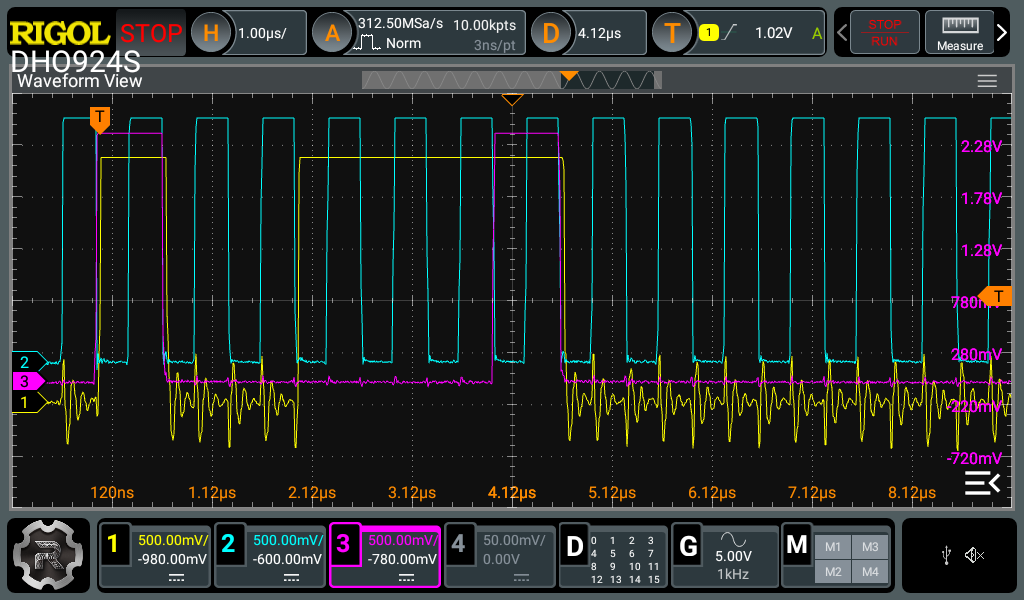
\includegraphics[width=\textwidth]{Pics/oszi_cube_spi_example.png}
	\caption{Screenshot des Osziloskopbildschirms. Dieser zeigt die Wellen für SCK (blau/türkis), MOSI (magenta) und MISO (gelb).}
	\label{fig:oszi_cube_spi_example}
\end{figure}

Mit den ersten Test wurden nur konnten SCK, MOSI und NSS (Negative Slave Select; andere Schreibweise für Chip Select) erfolgreich erzeugt werden.
Lediglich das MISO-Signale hatte nicht die erwartete Form.
Dieser Fehler rührte von einer falschen Einstellung des NSS Gpio-Objektes her.
Das Attribut \texttt{Alternate} war auf den Wert \texttt{None} eingestellt.
Damit hatte diese Objekt keine \textit{alternative} Funktion, wie sie für die Buskommunikation notwendig ist.
Nach der Korrektur des Objektes, konnte Schema der Signale aus \cref{fig:oszi_cube_spi_example} mit den neu erstellten Klassen rekonstruiert werden.
Das Ergebnis ist in \cref{fig:oszi_spi_signal_test} zu sehen.
Die dunkelblaue Linie zeigt das NSS-Signal, das hier nur auf dem Wert $0$ liegt.
Dessen Wechsel von $1$ auf $0$ liegt hier außerhalb des Sichfeldes.

\begin{figure}[H]
	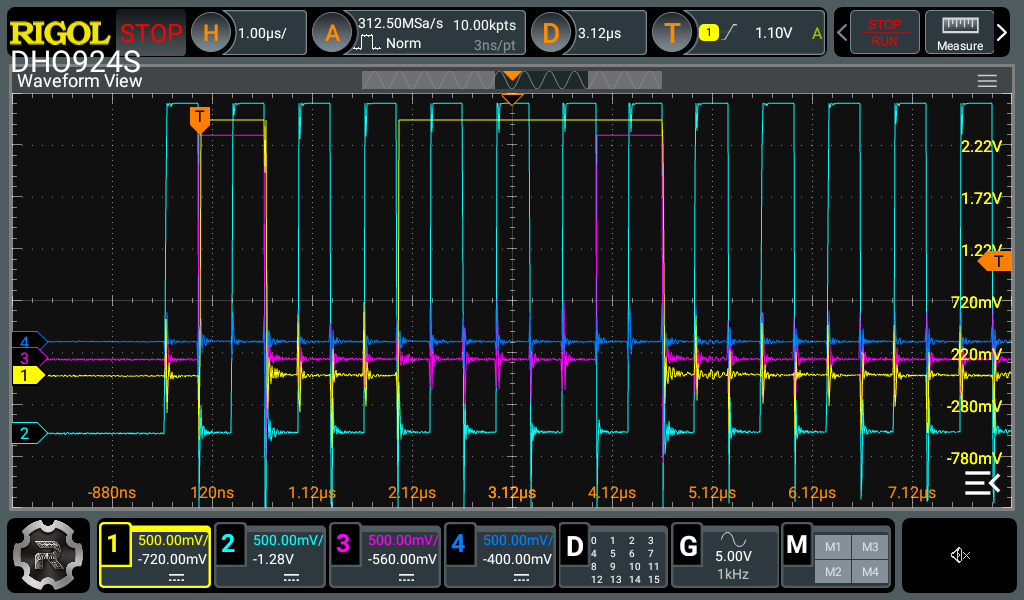
\includegraphics[width=\textwidth]{Pics/spi_signal_test.png}
	\caption{Screenshot einer erfolgreich SPI-Kommunikation, erstellt mit dem Code der HW\_API.}
	\label{fig:oszi_spi_signal_test}
\end{figure}


Die Testumgebung umfasste sowohl zwei Familien der STM32-Hardware (Nucleo-C031C6, Nucleo-G071RB, Nucleo-G0B1RE) als auch ein ESP32C6-DevKit, jeweils verbunden mit Debug-Schnittstellen und notwendiger Peripherie.
Die modulare Struktur, in der plattformspezifische Implementierungen klar gekapselt sind, ermöglicht neben der Übertragung der Lösung, auf unterschiedliche \gls{mcu}-Familien, ohne Anpassungen des Applikationscodes, auch die Erweiterung um fehlende Funktionsmodule oder neuer Microcontroller.
Einschränkungen bestehen lediglich in der begrenzten Testabdeckung, sowohl für STM32-Familien, als auch ESP32 Microcontroller, die nicht direkt validiert wurden.
% TODO: Dieser Absatz ans Ende der Validierung
Zusammenfassend zeigt die Validierung, dass die HW\_API die geforderten funktionalen Anforderungen erfüllt, korrekt arbeitet und eine stabile Grundlage für die Implementierung plattformunabhängiger Embedded-Anwendungen darstellt. 
Die gewählten Testmethoden gewährleisten eine nachvollziehbare und reproduzierbare Überprüfung der Softwarequalität.


\subsection{Weitere Erkenntnisse}
\begin{itemize}
	\item Größenänderung der Builddateien
	\item Komplexität der Funktionen $\rightarrow$ vgl. Cube
	\item 
\end{itemize}







































